%\documentstyle[epsf,twocolumn]{jarticle}       %LaTeX2e仕様
\documentclass[twocolumn]{jarticle}     %pLaTeX2e仕様(platex.exeの場合)
%\documentclass[twocolumn]{ujarticle}     %pLaTeX2e仕様(uplatex.exeの場合)
%%%%%%%%%%%%%%%%%%%%%%%%%%%%%%%%%%%%%%%%%%%%%%%%%%%%%%%%%%%%%%
%%
%%  基本バージョン
%%
%%%%%%%%%%%%%%%%%%%%%%%%%%%%%%%%%%%%%%%%%%%%%%%%%%%%%%%%%%%%%%%%
\setlength{\topmargin}{-45pt}
%\setlength{\oddsidemargin}{0cm} 
\setlength{\oddsidemargin}{-7.5mm}
%\setlength{\evensidemargin}{0cm} 
\setlength{\textheight}{24.1cm}
%setlength{\textheight}{25cm} 
\setlength{\textwidth}{17.4cm}
%\setlength{\textwidth}{172mm} 
\setlength{\columnsep}{11mm}

\kanjiskip=.07zw plus.5pt minus.5pt


% 【節が変わるごとに (1.1)(1.2) … (2.1)(2.2) と数式番号をつけるとき】
%\makeatletter
%\renewcommand{\theequation}{%
%\thesection.\arabic{equation}} %\@addtoreset{equation}{section}
%\makeatother

%\renewcommand{\arraystretch}{0.95} 行間の設定

%%%%%%%%%%%%%%%%%%%%%%%%%%%%%%%%%%%%%%%%%%%%%%%%%%%%%%%%
\usepackage[dvipdfmx]{graphicx}   %pLaTeX2e仕様(\documentstyle ->\documentclass)\documentclass[dvipdfmx]{graphicx}
\usepackage[dvipdfmx]{color}
\usepackage[subrefformat=parens]{subcaption}
\usepackage{colortbl}
\usepackage{multicol}
%%%%%%%%%%%%%%%%%%%%%%%%%%%%%%%%%%%%%%%%%%%%%%%%%%%%%%%%

\begin{document}

\twocolumn[
\noindent

\hspace{1em}
2020年12月25日
\hfill
\ \ 細川 岳大

\vspace{2mm}

\hrule

\begin{center}
{\Large \bf 進捗報告}
\end{center}
\hrule
\vspace{3mm}
]

% ‚ここから 文章 Start!

\section{今週やったこと}

\begin{itemize}
	\item GAの実験
\end{itemize}

\section{GAの実験}
表\ref{tb:GApara},\ref{tb:FTXpara}に実験の設定を示す.
遺伝子は0から9の整数値をとる整数値コーディングとした.\\
選択はサイズ2のトーナメント選択,交叉には二点交叉,突然変異は別の数値にランダムに移るように設定した.


また,今回は One-shot モデルを用いた.


\subsection{結果}
図\ref{fig:ex1}に示す.
結果として今回も正答数を上げるには至らなかった.
今までと同様の結果のため特に考察が出来るわけではないが,
val\ dataだけでなくtest\ dataに対する識別率も確認する必要があると思った.

\begin{figure}[h]
	\begin{center}
		\vspace*{-3mm}
		\hspace*{-12mm}
		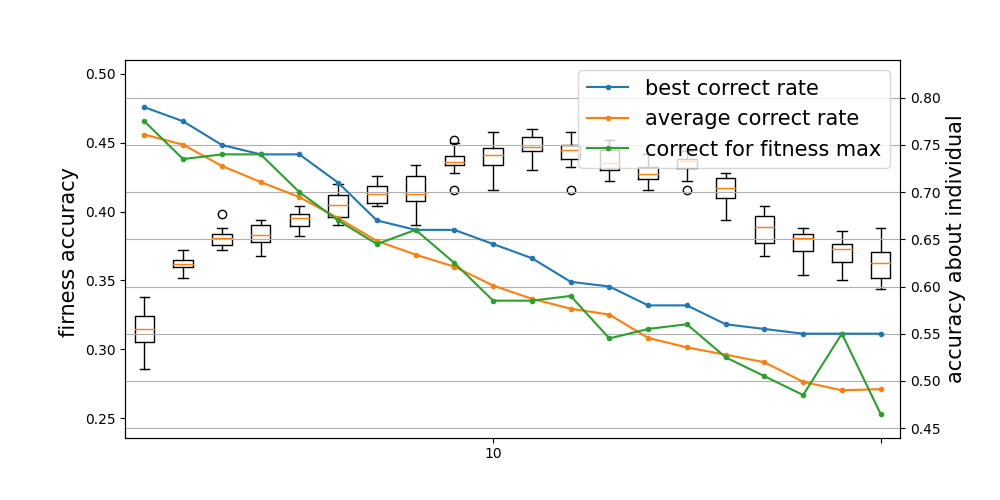
\includegraphics[height=65mm,width=100mm]{graph2.png}
		\caption{実験1の結果\label{fig:ex1}}
	\end{center}
\end{figure}

\section{来週の課題}
\begin{itemize}
	\item 実験設定の改良
	\item SimCLRを用いた実験
\end{itemize}


\begin{table}[h]
	\centering
	\caption{GAの設定\label{tb:GApara}}
	\scalebox{1.0}{
		\begin{tabular}{|c||c|} \hline
			個体数&20\\ \hline
			世代数&20\\ \hline
			交叉率&1.0\\ \hline
			突然変異率&0.03\\ \hline\hline
			labeled&250枚\\ \hline
			search&100枚\\ \hline
		\end{tabular}
	}
\end{table}

\begin{table}[h]
	\centering
	\caption{FixMatchの設定\label{tb:FTXpara}}
	\scalebox{1.0}{
		\begin{tabular}{|c|c|c|} \hline
			model&\multicolumn{2}{c|}{WideResNet16-2}\\ \hline\hline
			data set&\multicolumn{2}{c|}{cifar10}\\ \hline
			\multicolumn{3}{|c|}{事前学習}\\ \hline
			batch size&labeled&32\\ \cline{2-3}
			&unlabeled&$32*7$\\ \hline
			optimizer&\multicolumn{2}{c|}{SGD(lr=0.05,momntum=0.9)}\\ \hline
			train &labeled&100\\ \cline{2-3}
			&unlabeled&49650\\ \hline			
			val data&\multicolumn{2}{c|}{150}\\ \hline
			num\_iterations&\multicolumn{2}{c|}{2**16}\\ \hline\hline
			\multicolumn{3}{|c|}{GAの評価}\\ \hline
			batch size&labeled&32\\ \cline{2-3}
			&unlabeled&$32*2$\\ \hline
			optimizer&\multicolumn{2}{c|}{SGD(lr=0.003,momntum=0.9)}\\ \hline
			train &searchのみ&100\\ \cline{2-3}
			&unlabeled&49650\\ \hline
			val data&\multicolumn{2}{c|}{250}\\ \hline
			num\_iterations&1世代目&3000\\ \cline{2-3}
			&以降&500\\ \hline
		\end{tabular}
	}
\end{table}





\end{document}


